% Options for packages loaded elsewhere
\PassOptionsToPackage{unicode}{hyperref}
\PassOptionsToPackage{hyphens}{url}
%
\documentclass[
  english,
  ,man,floatsintext]{apa6}
\usepackage{lmodern}
\usepackage{amsmath}
\usepackage{ifxetex,ifluatex}
\ifnum 0\ifxetex 1\fi\ifluatex 1\fi=0 % if pdftex
  \usepackage[T1]{fontenc}
  \usepackage[utf8]{inputenc}
  \usepackage{textcomp} % provide euro and other symbols
  \usepackage{amssymb}
\else % if luatex or xetex
  \usepackage{unicode-math}
  \defaultfontfeatures{Scale=MatchLowercase}
  \defaultfontfeatures[\rmfamily]{Ligatures=TeX,Scale=1}
\fi
% Use upquote if available, for straight quotes in verbatim environments
\IfFileExists{upquote.sty}{\usepackage{upquote}}{}
\IfFileExists{microtype.sty}{% use microtype if available
  \usepackage[]{microtype}
  \UseMicrotypeSet[protrusion]{basicmath} % disable protrusion for tt fonts
}{}
\makeatletter
\@ifundefined{KOMAClassName}{% if non-KOMA class
  \IfFileExists{parskip.sty}{%
    \usepackage{parskip}
  }{% else
    \setlength{\parindent}{0pt}
    \setlength{\parskip}{6pt plus 2pt minus 1pt}}
}{% if KOMA class
  \KOMAoptions{parskip=half}}
\makeatother
\usepackage{xcolor}
\IfFileExists{xurl.sty}{\usepackage{xurl}}{} % add URL line breaks if available
\IfFileExists{bookmark.sty}{\usepackage{bookmark}}{\usepackage{hyperref}}
\hypersetup{
  pdftitle={Justify Your Alpha: A Practical Guide},
  pdflang={en-EN},
  pdfkeywords={hypothesis testing, Type 1 error, Type 2 error, statistical power},
  hidelinks,
  pdfcreator={LaTeX via pandoc}}
\urlstyle{same} % disable monospaced font for URLs
\usepackage{graphicx}
\makeatletter
\def\maxwidth{\ifdim\Gin@nat@width>\linewidth\linewidth\else\Gin@nat@width\fi}
\def\maxheight{\ifdim\Gin@nat@height>\textheight\textheight\else\Gin@nat@height\fi}
\makeatother
% Scale images if necessary, so that they will not overflow the page
% margins by default, and it is still possible to overwrite the defaults
% using explicit options in \includegraphics[width, height, ...]{}
\setkeys{Gin}{width=\maxwidth,height=\maxheight,keepaspectratio}
% Set default figure placement to htbp
\makeatletter
\def\fps@figure{htbp}
\makeatother
\setlength{\emergencystretch}{3em} % prevent overfull lines
\providecommand{\tightlist}{%
  \setlength{\itemsep}{0pt}\setlength{\parskip}{0pt}}
\setcounter{secnumdepth}{-\maxdimen} % remove section numbering
% Make \paragraph and \subparagraph free-standing
\ifx\paragraph\undefined\else
  \let\oldparagraph\paragraph
  \renewcommand{\paragraph}[1]{\oldparagraph{#1}\mbox{}}
\fi
\ifx\subparagraph\undefined\else
  \let\oldsubparagraph\subparagraph
  \renewcommand{\subparagraph}[1]{\oldsubparagraph{#1}\mbox{}}
\fi
% Manuscript styling
\usepackage{upgreek}
\captionsetup{font=singlespacing,justification=justified}

% Table formatting
\usepackage{longtable}
\usepackage{lscape}
% \usepackage[counterclockwise]{rotating}   % Landscape page setup for large tables
\usepackage{multirow}		% Table styling
\usepackage{tabularx}		% Control Column width
\usepackage[flushleft]{threeparttable}	% Allows for three part tables with a specified notes section
\usepackage{threeparttablex}            % Lets threeparttable work with longtable

% Create new environments so endfloat can handle them
% \newenvironment{ltable}
%   {\begin{landscape}\begin{center}\begin{threeparttable}}
%   {\end{threeparttable}\end{center}\end{landscape}}
\newenvironment{lltable}{\begin{landscape}\begin{center}\begin{ThreePartTable}}{\end{ThreePartTable}\end{center}\end{landscape}}

% Enables adjusting longtable caption width to table width
% Solution found at http://golatex.de/longtable-mit-caption-so-breit-wie-die-tabelle-t15767.html
\makeatletter
\newcommand\LastLTentrywidth{1em}
\newlength\longtablewidth
\setlength{\longtablewidth}{1in}
\newcommand{\getlongtablewidth}{\begingroup \ifcsname LT@\roman{LT@tables}\endcsname \global\longtablewidth=0pt \renewcommand{\LT@entry}[2]{\global\advance\longtablewidth by ##2\relax\gdef\LastLTentrywidth{##2}}\@nameuse{LT@\roman{LT@tables}} \fi \endgroup}

% \setlength{\parindent}{0.5in}
% \setlength{\parskip}{0pt plus 0pt minus 0pt}

% \usepackage{etoolbox}
\makeatletter
\patchcmd{\HyOrg@maketitle}
  {\section{\normalfont\normalsize\abstractname}}
  {\section*{\normalfont\normalsize\abstractname}}
  {}{\typeout{Failed to patch abstract.}}
\makeatother
\shorttitle{Justify in Practice}
\author{Maximilian Maier\textsuperscript{1}\ \& Daniel Lakens\textsuperscript{2}}
\affiliation{
\vspace{0.5cm}
\textsuperscript{1} University of Amsterdam, The Netherlands\\\textsuperscript{2} Eindhoven University of Technology, The Netherlands}
\authornote{All code used to create this manuscript is provided in an OSF repository at https://osf.io/h5e2q/.


Correspondence concerning this article should be addressed to Daniel Lakens, ATLAS 9.402, 5600 MB, Eindhoven, The Netherlands. E-mail: D.Lakens@tue.nl}
\keywords{hypothesis testing, Type 1 error, Type 2 error, statistical power\newline\indent Word count: 4890 words}
\usepackage{lineno}

\linenumbers
\usepackage{csquotes}
\ifxetex
  % Load polyglossia as late as possible: uses bidi with RTL langages (e.g. Hebrew, Arabic)
  \usepackage{polyglossia}
  \setmainlanguage[]{english}
\else
  \usepackage[shorthands=off,main=english]{babel}
\fi
\ifluatex
  \usepackage{selnolig}  % disable illegal ligatures
\fi
\newlength{\cslhangindent}
\setlength{\cslhangindent}{1.5em}
\newlength{\csllabelwidth}
\setlength{\csllabelwidth}{3em}
\newenvironment{CSLReferences}[2] % #1 hanging-ident, #2 entry spacing
 {% don't indent paragraphs
  \setlength{\parindent}{0pt}
  % turn on hanging indent if param 1 is 1
  \ifodd #1 \everypar{\setlength{\hangindent}{\cslhangindent}}\ignorespaces\fi
  % set entry spacing
  \ifnum #2 > 0
  \setlength{\parskip}{#2\baselineskip}
  \fi
 }%
 {}
\usepackage{calc}
\newcommand{\CSLBlock}[1]{#1\hfill\break}
\newcommand{\CSLLeftMargin}[1]{\parbox[t]{\csllabelwidth}{#1}}
\newcommand{\CSLRightInline}[1]{\parbox[t]{\linewidth - \csllabelwidth}{#1}\break}
\newcommand{\CSLIndent}[1]{\hspace{\cslhangindent}#1}

\title{Justify Your Alpha: A Practical Guide}

\date{}

\abstract{
The default use of an alpha level of 0.05 is sub-optimal for two reasons. First, decisions based on data can be made more efficiently by choosing an alpha level that minimizes the combined Type 1 and Type 2 error rate. Second, in studies with very high statistical power \emph{p}-values lower than the alpha level can actually be support for the null hypothesis, instead of for the alternative hypothesis. Because it is difficult to abandon a bad practice without providing an alternative, this manuscript explains two approaches that can be used to justify your alpha. The first approach is based on the idea to either minimize or balance Type 1 and Type 2 error rates. The second approach lowers the alpha level as a function of the sample size. Software is provided to perform the required calculations. Both approaches have their limitations (e.g., the challenge of specifying relative costs and priors, or the slightly arbitrary nature of how the alpha level should decrease as the sample size increases) but they nevertheless provide a clear improvement compared to current practices. The use of alpha levels that have a better justification should improve statistical inferences and increase the efficiency of scientific research.
}

\begin{document}
\maketitle

Researchers often rely on data to decide how to act. In a Neyman-Pearson approach to hypothesis testing (Neyman \& Pearson, 1933) studies are designed such that erroneous decisions that determine how we act are controlled in the long run at some desired maximum level. If resources were infinite we could collect so much data that the chance of making a wrong decision is incredibly small. But resources are often limited, which means that researchers need to decide how to choose the rate at which they are willing to make errors. After data is collected researchers can incorrectly act as if there is an effect when there is no true effect (a Type 1 error) or incorrectly act as if there is no effect when there is a true effect (a Type 2 error). For any fixed sample size and true effect size a reduction in the Type 1 error rate will increase the Type 2 error rate and vice versa.

The question how error rates should be set in any study requires careful consideration of the relative costs of a Type 1 error or a Type 2 error. Regrettably researchers rarely provide such a justification, and predominantly use a Type 1 error rate of 5\%. One reason researchers rely on norms instead of rationally chosen error rates is the absence of explanations how to justify a different alpha level than the normative use of 0.05. This article explains why error rates need to be justified, and provides two practical guidelines that can be used to justify the alpha level by balancing or minimizing error rates, or justify the alpha level by lowering it as a function of the sample size.

\hypertarget{why-do-we-use-a-5-alpha-level-and-80-power}{%
\section{Why do we use a 5\% alpha level and 80\% power?}\label{why-do-we-use-a-5-alpha-level-and-80-power}}

As a young scholar we might naively assume that when all researchers do something, there must be a good reason for such an established practice. An important step towards maturity as a scholar is the realization that this is not the case. Neither Fisher nor Neyman, two statistical giants largely responsible for the widespread reliance on hypothesis tests in the social sciences, recommended the universal use of any specific threshold. Fisher (1935) writes: ``It is open to the experimenter to be more or less exacting in respect of the smallness of the probability he would require before he would be willing to admit that his observations have demonstrated a positive result.'' Similarly, Neyman and Pearson (1933) write: ``From the point of view of mathematical theory all that we can do is to show how the risk of the errors may be controlled and minimized. The use of these statistical tools in any given case, in determining just how the balance should be struck, must be left to the investigator.''

Even though in theory alpha levels should be justified, in practice researchers tend to imitate others. Fisher writes in 1926: ``Personally, the writer prefers to set a low standard of significance at the 5 per cent point, and ignore entirely all results which fail to reach this level.'' This sentence is preceded by the statement ``If one in twenty does not seem high enough odds, we may, if we prefer it, draw the line at one in fifty (the 2 percent point), or one in a hundred (the 1 percent point).'' Indeed, in his examples Fisher often uses an alpha of 0.01. Nevertheless, researchers seem to have copied the value Fisher preferred, instead of his more important take-home message that the significance level should be set by the experimenter. The default use of an alpha level of 0.05 seems to originate from the early work of Gosset on the \emph{t}-distribution (Cowles \& Davis, 1982), who believed that a difference of two standard deviations (a z-score of 2) was sufficiently rare.

The default use of 80\% power (or a 20\% Type 2, or beta (b) error) is similarly based on personal preferences by Cohen (1988), who writes: ``It is proposed here as a convention that, when the investigator has no other basis for setting the desired power value, the value .80 be used. This means that beta is set at .20. This arbitrary but reasonable value is offered for several reasons (Cohen, 1965, pp.~98-99). The chief among them takes into consideration the implicit convention for alpha of .05. The beta of .20 is chosen with the idea that the general relative seriousness of these two kinds of errors is of the order of .20/.05, i.e., that Type I errors are of the order of four times as serious as Type II errors. This .80 desired power convention is offered with the hope that it will be ignored whenever an investigator can find a basis in his substantive concerns in his specific research investigation to choose a value ad hoc.''

We see that conventions are built on conventions: the norm to aim for 80\% power is built on the norm to set the alpha level at 5\%. However, the real lesson Cohen was teaching us is to determine the relative seriousness of Type 1 and Type 2 errors, and to balance both types of errors when a study is designed. If a Type 1 error is considered to be four times as serious as a Type 2 error, the \emph{weighted} error rates in the study are balanced. Instead of imitating the values chosen by Cohen, researchers should aim to imitate the approach he used to justify error rates.

\hypertarget{why-error-rates-should-be-justified}{%
\subsection{Why error rates should be justified}\label{why-error-rates-should-be-justified}}

In 1957 Neyman wrote: ``it appears desirable to determine the level of significance in accordance with quite a few circumstances that vary from one particular problem to the next.'' The mindless application of null hypothesis significance tests, including setting the alpha level at 5\% for all tests, has been criticized for more than half a century (Bakan, 1966; Gigerenzer, 2018). But it is difficult to abandon a mediocre research practice without an alternative.

There are two main reasons to abandon the universal use of a 5\% alpha level. The first reason to carefully choose an alpha level is that decision making becomes more efficient. If researchers use hypothesis tests to choose how to act while balancing error rates it is typically possible to make decisions more efficiently by setting the alpha level at a different value than 0.05. If we aim to either minimize or balance Type 1 and Type 2 error rates for a given sample size and effect size, the alpha level should be set not based on convention, but by weighting the relative costs of both types of errors.

The second reasons is that as the statistical power increases, some \emph{p}-values below 0.05 (e.g., \emph{p} = 0.04) can be more likely when there is \emph{no} effect than when there \emph{is} an effect. This is known as Lindley's paradox (Cousins, 2017; Lindley, 1957). The distribution of \emph{p}-values is a function of the statistical power (Cumming, 2008), and the higher the power, the more right-skewed the distribution becomes (i.e.~the more low \emph{p}-values are observed). When there is no true effect \emph{p}-values are uniformly distributed, and 1\% of observed \emph{p}-values fall between 0.04 and 0.05. When the statistical power is extremely high, not only will most \emph{p}-values fall below 0.05, most will also fall below 0.01. In Figure \ref{fig:p-plot} we see that with high power very low \emph{p}-values are more likely to be observed when there \emph{is} an effect than when there is \emph{no} effect (e.g., the black curve representing \emph{p}-values when the alternative is true falls above the dashed horizontal line for a \emph{p}-value of 0.01). But observing a \emph{p}-value of 0.04 is more likely when the null hypothesis is true than when the alternative hypothesis is true and we have very high power (the horizontal dashed line falls above the black curve for \emph{p}-values larger than \textasciitilde0.025).

\begin{figure}
\centering
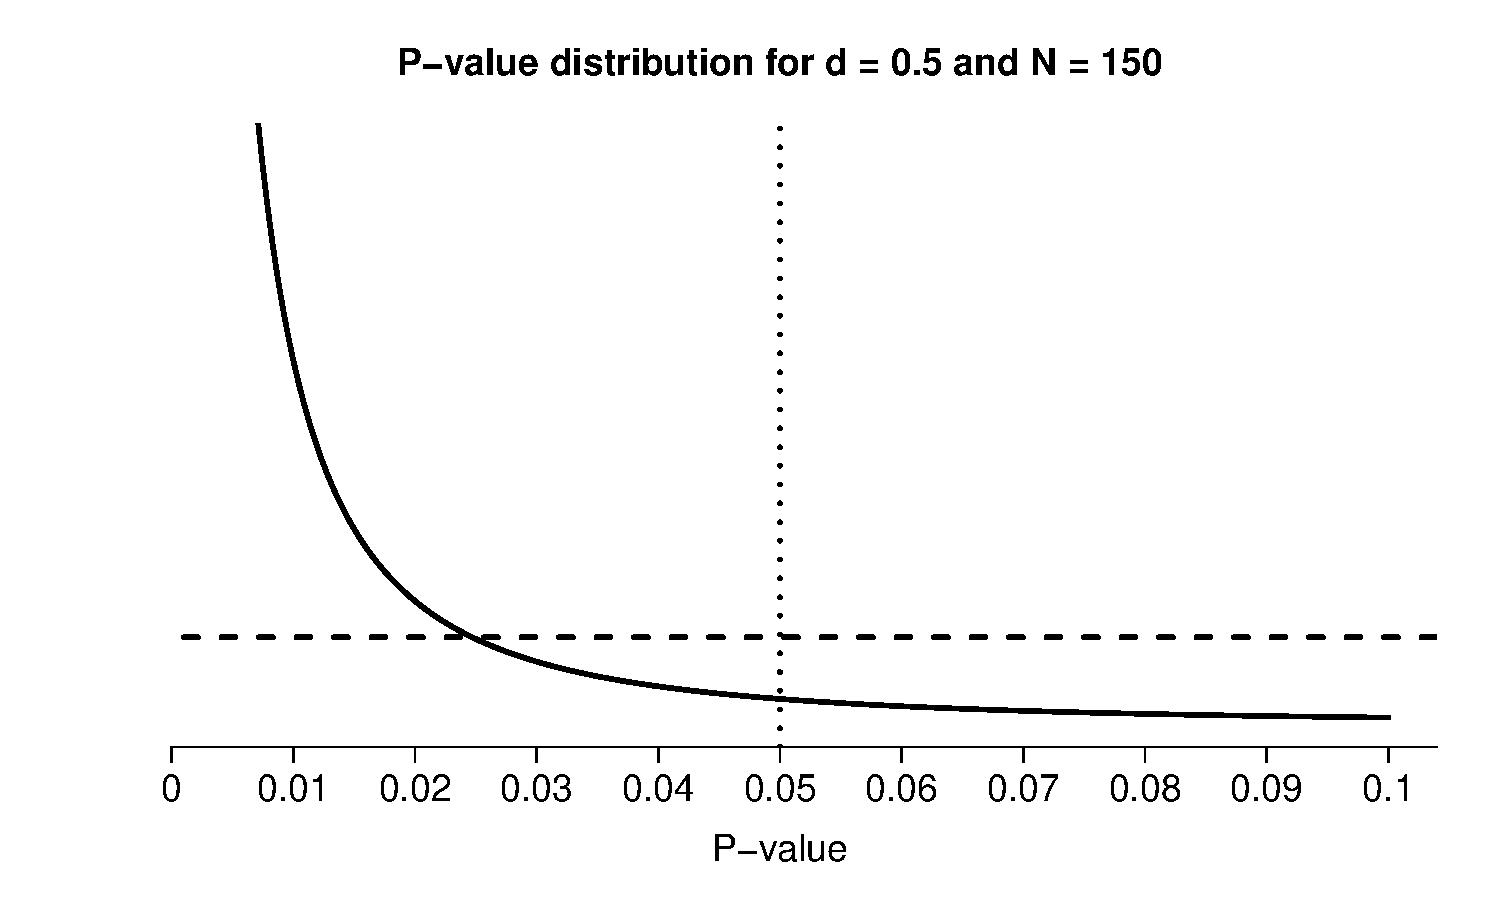
\includegraphics{Justify_in_Practice_files/figure-latex/p-plot-1.pdf}
\caption{\label{fig:p-plot}\emph{P}-value distributions for a two-sided independent \emph{t}-test with N = 150 and d = 0.5 (black curve) or d = 0 (horizontal dashed line) which illustrates how \emph{p}-values just below 0.05 can be more likely when there is no effect than when there is an effect.}
\end{figure}

Researchers often want to interpret a significant test result as `support' for the alternative hypothesis. If so, it makes sense to choose the alpha level such that when a significant \emph{p}-value is observed, the \emph{p}-value is actually more likely when the alternative hypothesis is true than when the null hypothesis is true. This means that when statistical power is very high (e.g., the sample size is very large), the alpha level should be reduced. For example, if the alpha level in Figure \ref{fig:p-plot} is lowered to 0.02 then the alternative hypothesis is more likely than the null hypothesis for all significant \emph{p}-values that would be observed.

\hypertarget{minimizing-or-balancing-type-1-and-type-2-error-rates}{%
\subsection{Minimizing or Balancing Type 1 and Type 2 Error Rates}\label{minimizing-or-balancing-type-1-and-type-2-error-rates}}

If both Type 1 as Type 2 errors are costly, then it makes sense to optimally reduce both errors as you design studies. This would make decision making overall most efficient. Researchers can choose to design a study with a statistical power and alpha level that minimize the \emph{combined error rate}. For example, assuming H0 and H1 are a-priori equally probable, with a 5\% alpha level and a statistical power of 80\% the combined error rate is (5 + 20)/2 = 12.5\%. If the statistical power is 99\% and the alpha is 5\% the combined error rate is (1 + 5)/2 = 3\%. As shown below, this approach can be extended to incorporate different prior probabilities of H0 and H1. Mudge, Baker, Edge, and Houlahan (2012) show that by choosing an alpha level based on the relative weight of Type 1 errors and Type 2 errors, and assuming beliefs about the prior probability that H0 and H1 are correct, decisions can be made more efficiently compared to the default use of an alpha level of 0.05.

Winer (1962) writes: ``The frequent use of the .05 and .01 levels of significance is a matter of convention having little scientific or logical basis. When the power of tests is likely to be low under these levels of significance, and when Type 1 and Type 2 errors are of approximately equal importance, the .30 and .20 levels of significance may be more appropriate than the .05 and .01 levels.'' The reasoning here is that a design that has 70\% power for the smallest effect size of interest would not balance the Type 1 and Type 2 error rates in a sensible manner. Similarly, in huge datasets it might be possible to achieve very high levels of power for all effect sizes that are still considered meaningful. If such a study has 99\% power for effect sizes of interest, and thus a 1\% Type 2 error rate, but uses a 5\% alpha level, it also suffers from a lack of balance. A common example of this latter scenario is the default use of a 5\% alpha level in meta-analyses, which often have extremely high power for any effect size that would be considered meaningful, and where it seems sensible to lower the alpha level considerably.

Researchers can decide to either balance Type 1 and Type 2 error rates (e.g., setting both at 5\%), or minimize error rates. For any given sample size and effect size of interest there is an alpha level that minimizes the combined error rates. Because the chosen alpha level also influences the statistical power, and the Type 2 error rate is therefore dependent upon the Type 1 error rate, minimizing or balancing error rates requires an iterative procedure. Imagine researchers plan to perform a study which will be analyzed with an independent two-sided \emph{t}-test. They initially plan to collect 50 participants per condition, and set their smallest effect size of interest to d = 0.5. They think a Type 1 error is just as severe as a Type 2 error, and believe H0 is just as likely to be true as H1. The combined error rate is minimized when they set alpha to 0.13 (see Figure \ref{fig:weight-plot}, dotted line), which will give the study a Type 2 error rate of beta = 0.166 to detect effects of d = 0.5. The combined error rate is 0.148, while it would have been 0.177 if the alpha level was set at 5\%\footnote{For the same scenario, balanced error rates are alpha = 0.149 and beta = 0.149.}. Instead of choosing an example that is more extreme, I think it is important to point out that a better justified alpha level not necessarily means a hugely different alpha level. The absolute benefits are more noticeable for study designs where Type 2 error rates are high when a 5\% alpha level would be used, or where the Type 2 error is very small and the alpha level can be reduced from 0.05. Similarly, Figure \ref{fig:weight-plot} shows that if one were to use an alpha level of 0.005 following recommendations of Benjamin et al. (2018) when collecting a sample size of 100 per group to detect an effect of d = 0.5, the study would be much less efficient than it could be if a higher alpha level is chosen. The more important take-home message is that, perhaps counter-intuitively, decision making is sometimes slightly more efficient after \emph{increasing} the alpha level from the default of 0.05.

\begin{figure}
\centering
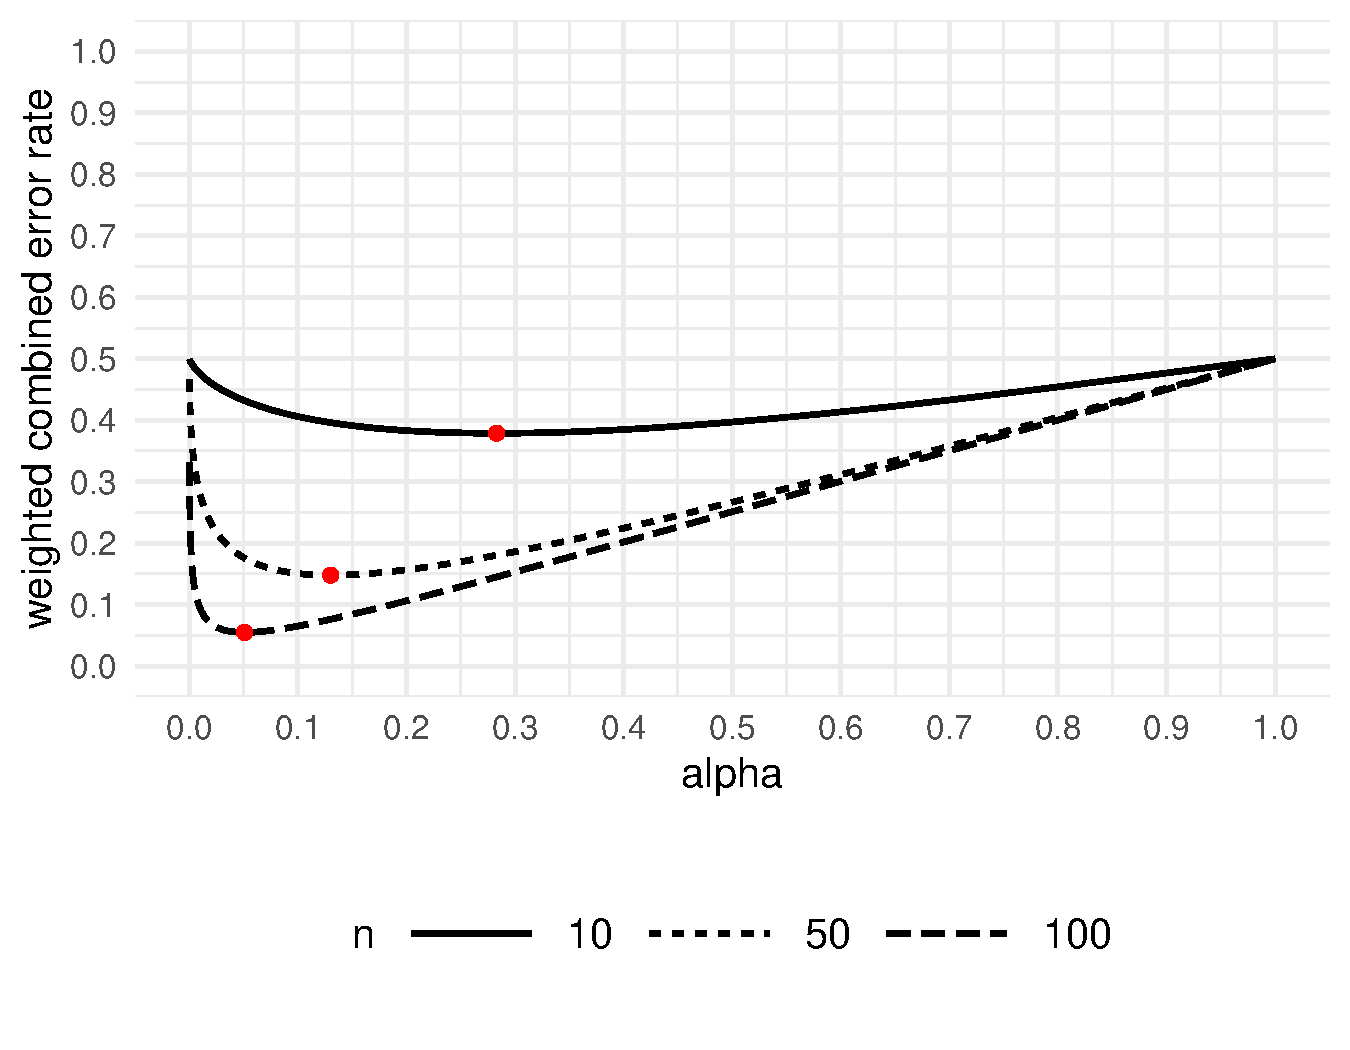
\includegraphics{Justify_in_Practice_files/figure-latex/weight-plot-1.pdf}
\caption{\label{fig:weight-plot}Weighted combined error rate (y-axis) for an independent \emph{t}-test with n = 10, n = 50, and n = 100 per group and a smallest effect of interest of d = 0.5, for all possible alpha levels (x-axis).}
\end{figure}

\hypertarget{weighing-the-relative-cost-of-errors}{%
\subsubsection{Weighing the Relative Cost of Errors}\label{weighing-the-relative-cost-of-errors}}

Cohen (1988) considered a study design with a 5\% Type 1 error rate and a 20\% Type 2 error rate balanced. The reason for this was that instead of weighing both types of errors equally, he felt ``Type I errors are of the order of four times as serious as Type II errors.'' To determine the relative costs of Type 1 and Type 2 errors researchers should perform a cost-benefit analysis. As an example from another discipline, (\textbf{field\_minimizing\_2004?}) quantify the relative costs of Type 1 errors when testing whether native species in Australia are declining. They come to the conclusion that when it comes to the Koala population, given its great economic value, a cost-benefit analysis indicates the alpha level should be set to 1. In other words, one should always act as if the population is declining, because the relative cost of a Type 2 error compared to a Type 1 error is extremely large.

Although it can be difficult to formally quantify all factors that determine the costs of Type 1 and Type 2 errors, there is no reason to let the perfect be the enemy of the good. In research questions where there are no direct applications of the research findings, relative costs might be largely subjective. If you have a research strategy where you always follow up on an initial study testing a theoretical prediction with a replication and extension study, and want to innovate, you might want to weigh a Type 2 error more strongly than a Type 1 error. If you are relatively sure policies will be changed based on the outcome of your single study, or it is unlikely many researchers will have the resources to replicate your study, a Type 1 error rate might be weighed more strongly than a Type 2 error. There are no right or wrong answers, but you need to think through this question when you design a study.

If we adapt our calculations for the example above where researchers who plan to collect 50 participants per condition to detect a d = 0.5 effect, but now weigh the cost of Type 1 errors 4 times as much as Type 2 errors, balanced error rates are alpha = 0.0654 and beta = 0.262. You will notice this is exactly the scenario Cohen describes, where a 5\% Type 1 error rate and 20\% Type 2 error rate is deemed a balanced design because Type 1 errors are weighed 4 times as much as Type 2 errors.

One could also aim to minimize error rates in the latter scenario by setting alpha to 0.0387 and beta to 0.343. Remember the cost of a Type 1 error is twice as large as the cost of a Type 1 error. Imagine a Type 1 error has a cost of 400 and a Type 2 error has a cost of 100. We perform 100 studies, 50 where H0 is true and 50 where H1 is true. We will make 1.93 Type 1 errors and 17.14 Type 2 errors, with a respective cost of 773.6 and 1714, respectively. Increasing or decreasing the alpha level for this design will only increase the total cost of errors, assuming H0 and H1 are equally probable. Figure \ref{fig:cost-plot} visualizes the weighted combined error rate for this study design across the all possible alpha levels.

\begin{figure}
\centering
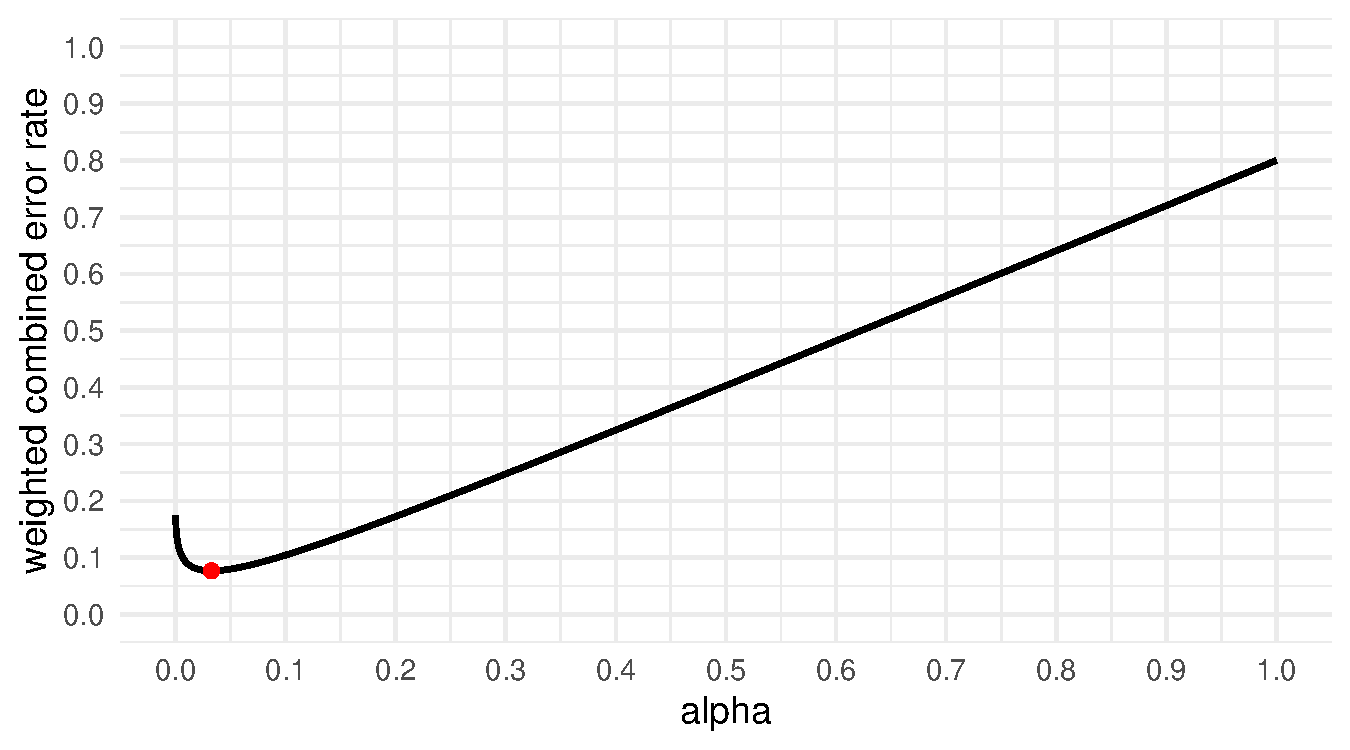
\includegraphics{Justify_in_Practice_files/figure-latex/cost-plot-1.pdf}
\caption{\label{fig:cost-plot}Weighted combined error rate (y-axis) for an independent \emph{t}-test with n = 50 per group and a smallest effect of interest of d = 0.5, where Type 1 errors are weighed 4 times as much as Type 2 errors, for all possible alpha levels (x-axis).}
\end{figure}

\hypertarget{incorporating-prior-probabilities}{%
\subsubsection{Incorporating prior probabilities}\label{incorporating-prior-probabilities}}

Miller and Ulrich (2019) explain how the choice for an optimal alpha level depends not just on the relative costs of Type 1 and Type 2 errors, but also on the base rate of true effects. In the extreme case, all studies a researcher designs test true hypotheses. In this case, there is no reason to worry about Type 1 errors, because a Type 1 error can only happen when the null hypothesis is true. Therefore, you can set the alpha level to 1 without any negative consequences. If the base rate of true hypotheses is very low, in the long run you will make many more Type 1 errors than Type 2 errors. For example, if you perform 1000 studies, and the base rate of true effects is 10\%, with 5\% Type 1 error rate and a 5\% Type 2 error rate you will observe 1000 × 0.9 × 0.05 = 45 Type 1 errors, and 1000 × 0.1 × 0.05 = 5 Type 2 errors. If possible, researchers can take their expectations about the long run frequency of Type 1 and Type 2 errors into account when choosing an alpha level that either balances or minimizes the error rates.

If you want to balance or minimize error rates in the long run, you should lower the alpha level as the prior probability of a null effect increases, or increase the alpha level as the prior probability of a true effect increases. Because the base rate of true hypotheses is unknown, this step requires subjective judgment. This can not be avoided, because one always makes assumptions about base rates, even if the assumption is that a hypothesis is equally likely to be true as false (with both H1 and H0 having a 50\% probability). Assuming equal prior probabilities for H1 and H0, we saw above that balanced error rates assuming d = 0.5 and collection n = 50 per condition in a \emph{t}-test would imply alpha = 0.149 and beta = 0.149. If you assume the null hypothesis is 10 times more likely than the alternative hypothesis (or the alternative hypothesis is 0.1 times as likely as the null hypothesis) then balanced error rates would require setting alpha to 0.0356 and beta to 0.355. If you believe the alternative hypothesis is twice as likely to be true as the null hypothesis, balancing error rates in the long run would mean increasing the alpha level and increasing the power by choosing alpha = 0.213 and beta = 0.107.

The two approaches (balancing error rates or minimizing error rates) typically yield quite similar results. Where minimizing error rates might be slightly more efficient, balancing error rates might be slightly more intuitive (especially when the prior probability of H0 and H1 are equal). Note that although there is always an optimal choice of the alpha level, there is always a range of values that yield quite similar weighted error rates. It is useful to plot weighted error rates as in Figure \ref{fig:cost-plot}. To balance or minimize error rates, researchers need to carefully consider the relative cost of Type 1 and Type 2 errors, the prior probability the null hypothesis is true, and the effect size they want to detect (Mudge, Baker, Edge, \& Houlahan, 2012), because these factors are used to calculate the weighted combined error rates \emph{w}:

\begin{equation}
\frac{(cost_{T1T2} \times \alpha + prior_{H1H0} \times \beta)}{prior_{H1H0}+cost_{T1T2}}
\label{eq:minimize}
\end{equation}

For example, imagine Type 1 errors are weighted 4 times as much as Type 2 errors (\(cost_{T1T2}\) = 4) and the alternative hypothesis is believed to be 2 times as likely as the null hypothesis (\(prior_{H1H0}\) = 10). With alpha = 0.213 and beta = 0.107 the weighted combined error rate is 0.142.

\hypertarget{sample-size-justification-when-minimizingbalancing-error-rates}{%
\subsubsection{Sample Size Justification when Minimizing/Balancing Error Rates}\label{sample-size-justification-when-minimizingbalancing-error-rates}}

So far we have only considered cases, where researchers wanted to justify their alpha level on a fixed sample size. However, in practice researchers should justify their sample size before running a study. The approach of balancing or minimizing error rates can straightforwardly be generalized to a sample size justification. To do so researchers need to specify the weighted combined error rate they are aiming for. The required sample size, significance level, and power can be determined accordingly.

Let us illustrate this using the example of researchers studying an effect of \emph{d} = 0.5 with a two sample \emph{t}-test. We can estimate the sample size as well as the alpha and power they would require to achieve a weighted combined error rate of 5\% when weighting Type 1 errors and Type 2 errors equally strong. Figure \ref{fig:error-plot} shows alpha, beta, and the weighted combined error rate as a function of sample size when the alpha level is minimized. We can see that a weighted combined error rate of 5\% (red line) is achieved at a sample size of 105. By iteratively optimizing the alpha level for different sample sizes and stopping when the desired error rate is reached, we can justify our sample size and the alpha level at the same time.

\begin{figure}
\centering
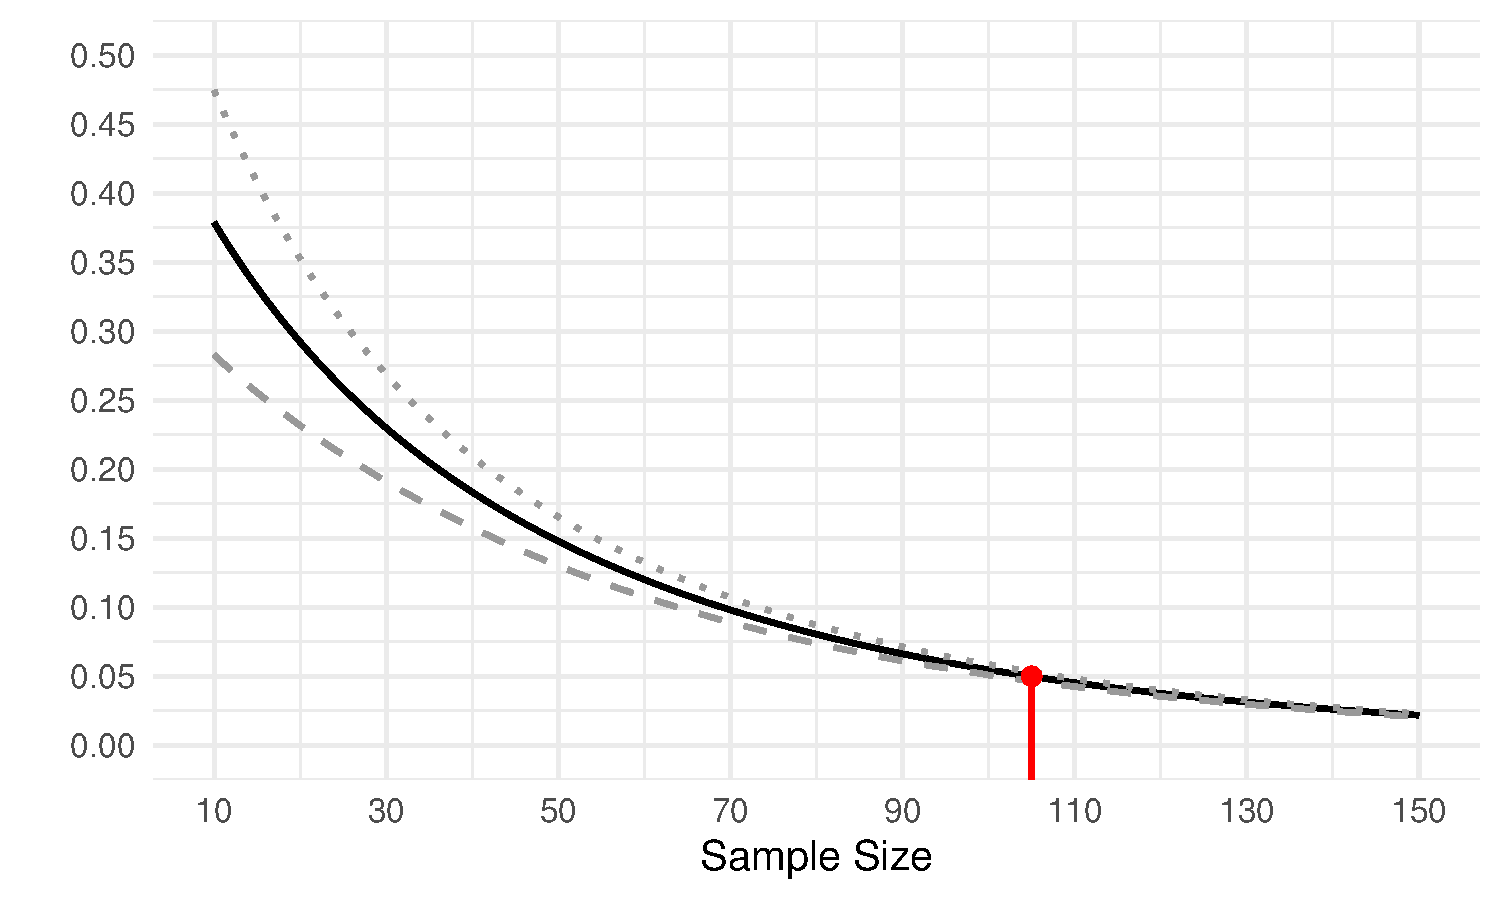
\includegraphics{Justify_in_Practice_files/figure-latex/error-plot-1.pdf}
\caption{\label{fig:error-plot}Weighted combined error rate (black), alpha (green), and beta (blue) for an independent \emph{t}-test as a function of sample size when the alpha level is justified to achieve lowest errors at each sample size.}
\end{figure}

\hypertarget{lowering-the-alpha-level-as-a-function-of-the-sample-size}{%
\subsection{Lowering the Alpha Level as a Function of the Sample Size}\label{lowering-the-alpha-level-as-a-function-of-the-sample-size}}

Sometimes a researcher might feel it is too challenging to specify relative costs, prior probabilities, and the effect size of interest, and be tempted to fall back to the use of an alpha level of 0.05. For such cases an approach exists where the alpha level is lowered as a function off the sample size. The need to do so is discussed extensively by Leamer (1978). He writes ``The rule of thumb quite popular now, that is, setting the significance level arbitrarily to .05, is shown to be deficient in the sense that from every reasonable viewpoint the significance level should be a decreasing function of sample size.'' This was already recognized by Harold Jeffreys (1939), who discusses ways to set the alpha level in the Neyman-Pearson approach to statistics: ``We should therefore get the best result, with any distribution of alpha, by some form that makes the ratio of the critical value to the standard error increase with n.~It appears then that whatever the distribution may be, the use of a fixed \emph{P} limit cannot be the one that will make the smallest number of mistakes.'' Good (1992) notes: ``we have empirical evidence that sensible \emph{P} values are related to weights of evidence and, therefore, that \emph{P} values are not entirely without merit. The real objection to \emph{P} values is not that they usually are utter nonsense, but rather that they can be highly misleading, especially if the value of N is not also taken into account and is large.''

To understand these recommendations it is important to distinguish between statistical inferences based on error control and inferences based on likelihoods. An alpha level of 5\% will limit incorrect decisions to a desired maximum (in the long run, and when all test assumptions are met). However, from a likelihood perspective it is possible that the observed data is much more likely when the null hypothesis is true, than when the alternative hypothesis is true, even when the observed \emph{p}-value is smaller than 0.05. This situation, known as Lindley's paradox, is visualized in Figure \ref{fig:p-plot}. It emerges because the critical value of a frequentist test approaches a limit as the sample size increases (e.g., \emph{t} = 1.96 for a two-sided \emph{t}-test). In Bayesian statistics the same Bayes factor requires a larger test statistic when the sample size is larger (see Jeffrey N. Rouder, Speckman, Sun, Morey, and Iverson (2009) and Zellner (1971)).

To prevent Lindley's paradox when using frequentist statistics one would need to adjust the alpha level in a way that the likelihood ratio (also called the Bayes factor) at the critical test statistic is always one. With such an alpha level, a significant \emph{p}-value will always be as least as likely if the alternative is true than if the null is true, successfully avoiding the Lindley paradox. Faulkenberry (2019) and Jeffrey N. Rouder, Speckman, Sun, Morey, and Iverson (2009) developed Bayes factors for \emph{t}-tests and ANOVAs which can calculate the Bayes factor from the test statistic and degrees of freedom.
Based on these papers we developed a shiny app (link) to reduce the alpha level proportional to the sample size and avoid Lindley's paradox. However, it can be considered evenly paradoxical to reject the null hypothesis even so the evidence for the alternative from a Bayesian point of view is only weak as the case with a likelihood ratio of one. To reliably avoid false positives one would need a tool in which a significant \emph{p}-value corresponds to moderate or strong evidence from a likelihoodist or Bayesian perspective. As a rule of thumb, if the data is 3 to 10 times more likely under the alternative than under the null this is considered moderate evidence, and data more than 10 times more likely under the alternative is considered strong evidence (H. Jeffreys, 1939, Appendix 1; Lee \& Wagenmakers, 2013, p. 105). Therefore, we extended the shiny app to also allow researchers to adjust the alpha level in a way that a significant \emph{p}-value will always provide moderate or strong evidence against the null hypothesis.

Our calculations are based on a unit information prior.\footnote{For t-tests the shiny app also allows to use the more common Cauchy prior.} This prior is relatively wide which sometimes results in overstated evidence for H0. However, while it is usually wise to use more informed priors (e.g., McElreath, 2020), we believe that to avoid the Lindley paradox a wide prior is the more conservative choice. In other words, it will prevent overstating the evidence for H1 and consequently be more likely to use an alpha level that is too low, rather than an alpha level that is too high. In addition, in contrast to previous approaches that aimed to calculate a Bayes factor for every \emph{p}-value (Colquhoun, 2017; e.g., D. Colquhoun, 2019) our application does not require researchers to specify the effect size under the alternative. Although the unit information prior is still an expectation for H1, not needing to specify the prior directly will likely increase the adoption among empirical researchers who sometimes find it difficult to specify a smallest effect size of interest or an expected effect size.

Let us illustrate this using one example study from the Deryl Bem's infamous paper on `'feeling the future'' (Bem, 2011). In this paper Derly Bem claimed in a series of 9 studies that he found evidence for a phenomenon called \emph{psi} which allows humans to predict the future. The publication of this implausible result in a well-known psychological journal, has sparked wide spread discussion about the replicability and data anlysis practices in psychology Galak, LeBoeuf, Nelson, \& Simmons (2012).

In study six of his paper, Bem reports the following one sample \emph{t}-tests \(t\)(149) = 1.80, \(p\) = .037, \(d\) = 0.15, \(p\) = .041 and \(t\)(149) = 1.77, \(p\) = .039, \(p\) = .041, as evidence for `'retroactive habituation''. It seems like the \(p\)-values in this study are remarkably close to the 5\% threshold, especially given the high sample size. Therefore, let us consider which alpha level Bem would have needed to use to avoid Lindley's Paradox, and to achieve moderate or strong evidence.

To avoid Lindley's paradox, Bem would need to use an alpha level of 0.0274. In other words, the observed \emph{p}-value is more likely under the null hypothesis than under the alternative. However, it seems desirable to require at least moderate evidence for the alternative before claiming a discovery. To achieve this Bem would have needed to use a alpha level of 0.0077. To provide strong evidence given a significant \emph{p}-value, he would have needed to use an even lower alpha level of 0.0020. We can see from this example, that \emph{p} = 0.05 is too low of an evidential standard under large sample sizes.

Although in principle for small sample sizes the function could return an alpha level \emph{larger} than 0.05, this is not the intended use. The reason for this is that we do not aim to replace the frequentist error rates with likelihood ratios but merely to reliably identify the cases where both approaches to statistical inference come to the same conclusions.

\hypertarget{comparison-of-the-two-approaches}{%
\subsection{Comparison of The Two Approaches}\label{comparison-of-the-two-approaches}}

When should we minimize or balance error rates and when should we avoid the Lindley paradox? In practice, it might be most convenient to use the first approach, whenever there is enough information to conduct power analysis, and if not to fall back on the second approach. Alternatively, one can also apply both approaches and choose the one that is more conservative (i.e., results in a lower alpha level). In addition, researchers aiming to find a compromise between Frequentist and Bayesian inference might be drawn more strongly towards the second approach (e.g., Good, 1992).

Figure \ref{fig:heatmap} shows which alpha level is larger as a function of sample size (per group) and expected effect size for a two-sample \emph{t}-test. For green values minimizing error rates resulted in higher alpha values, whereas red areas mean that avoiding the Lindley paradox resulted in higher alpha levels. We can see that when the expected effect size increases (x-axis) the alpha level will be smaller when using the method that minimizes error rates. This is mostly a result of how we set up the likelihood ratio calculations. Due to the unit information prior the method trying to avoid the Lindley paradox is not sensitive to the expected effect size. If the sample size increases on the other hand (y-axis) the alpha level reduces faster when avoiding the Lindley paradox then when minimizing error rates.

\begin{figure}
\centering
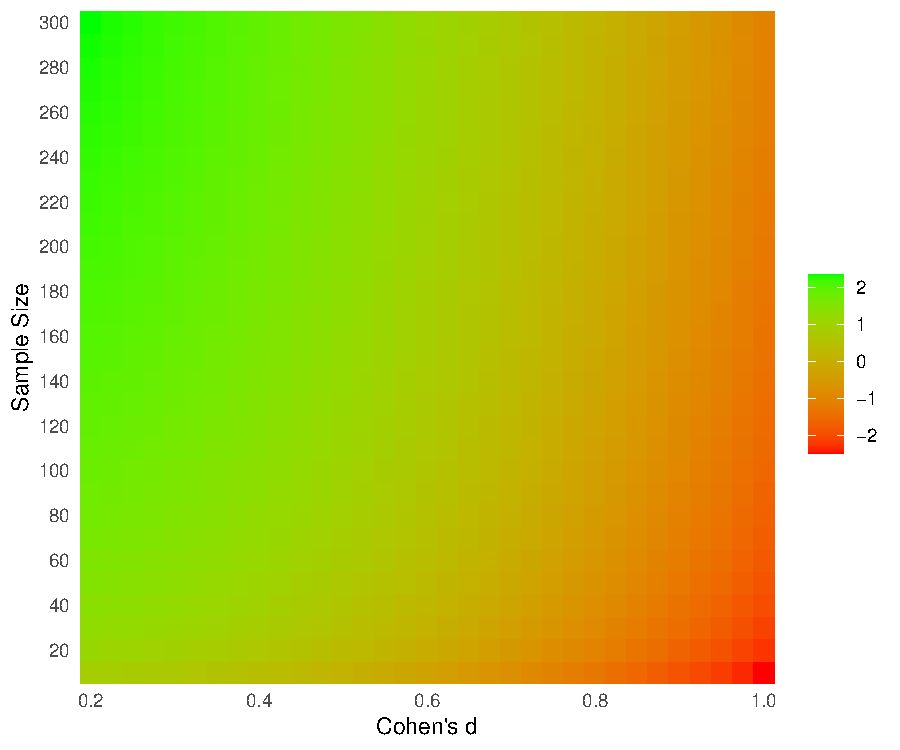
\includegraphics{Justify_in_Practice_files/figure-latex/heatmap-1.pdf}
\caption{\label{fig:heatmap}Heatmap of log(alpha\_minimize/alpha\_lindley) as a function of sample size and expected effect size.}
\end{figure}

\hypertarget{discussion}{%
\section{Discussion}\label{discussion}}

Editors and reviewers should \emph{always} ask authors to justify their choice of error rates, whenever researchers use data to make decisions about the presence or absence of an effect. As Skipper, Guenther, and Nass (1967) remarks: ``If, in contrast with present policy, it were conventional that editorial readers for professional journals routinely asked:''What justification is there for this level of significance? authors might be less likely to indiscriminately select an alpha level from the field of popular eligibles." In a Neyman-Pearson approach to statistics, the alpha level should be set before the data is collected. When reviewers of for example a Registered Report would ask authors to justify their alpha level, it would be convenient if they can recommend some approaches to do so. The current manuscript hopefully helps to fill this gap.

If a power analysis can be performed (i.e., whenever a desired or expected effect size of interest can be specified) and relative costs and priors can be specified, researchers can design efficient by minimizing or balancing error rates, optimizing informational value, or aiming for specific posterior probabilities. If it is difficult to specify these aspects of the study, researchers can fall back to the approach where the alpha level is reduced as a function of the sample size.

A Shiny app is available that allows users to perform the calculations recommended in this article. It can be used to minimize or balance alpha and beta, which works by specifying the effect size of interest and the sample size, as well as an analytic power calculation. The effect size should be determined as in a normal a-priori power analysis (preferably based on the smallest effect size of interest, for recommendations, see Albers and Lakens (2018)). Alternatively, researchers lower the alpha level as a function of the sample size by specifying only their sample size. Whichever approach is used, it is strongly recommended to preregister the alpha level that researchers plan to use before the data is collected.

Because of the strong overreliance on a 5\% error rate when designing studies, we have seen relatively few people attempt to justify their alpha level. As researchers start to justify their alpha, we will hopefully see the development of good examples and best practices for psychological science. It might be a challenge to get started, but the two approaches presented in the current article are one way to move away from the mindless use of a 5\% alpha level. There is a lot to gain, and justifying alpha levels should improve our statistical inferences and increase the efficiency of the research we perform.

\hypertarget{references}{%
\section{References}\label{references}}

\setlength{\parindent}{-0.5in}
\setlength{\leftskip}{0.5in}

\hypertarget{refs}{}
\begin{CSLReferences}{1}{0}
\leavevmode\hypertarget{ref-albers_when_2018}{}%
Albers, C., \& Lakens, D. (2018). When power analyses based on pilot data are biased: {Inaccurate} effect size estimators and follow-up bias. \emph{Journal of Experimental Social Psychology}, \emph{74}, 187--195. \url{https://doi.org/10.1016/j.jesp.2017.09.004}

\leavevmode\hypertarget{ref-bakan_test_1966}{}%
Bakan, D. (1966). The test of significance in psychological research. \emph{Psychological Bulletin}, \emph{66}(6), 423--437.

\leavevmode\hypertarget{ref-bem2011feeling}{}%
Bem, D. J. (2011). Feeling the future: Experimental evidence for anomalous retroactive influences on cognition and affect. \emph{Journal of Personality and Social Psychology}, \emph{100}(3), 407.

\leavevmode\hypertarget{ref-bem2011feeling}{}%
Bem, D. J. (2011). Feeling the future: Experimental evidence for anomalous retroactive influences on cognition and affect. \emph{Journal of Personality and Social Psychology}, \emph{100}(3), 407.

\leavevmode\hypertarget{ref-benjamin_redefine_2018}{}%
Benjamin, D. J., Berger, J. O., Johannesson, M., Nosek, B. A., Wagenmakers, E.-J., Berk, R., \ldots{} Johnson, V. E. (2018). Redefine statistical significance. \emph{Nature Human Behaviour}, \emph{2}(1), 6--10. \url{https://doi.org/10.1038/S41562-017-0189-Z}

\leavevmode\hypertarget{ref-cohen_statistical_1988}{}%
Cohen, J. (1988). \emph{Statistical power analysis for the behavioral sciences} (2nd ed). {Hillsdale, N.J}: {L. Erlbaum Associates}.

\leavevmode\hypertarget{ref-colquhoun2017reproducibility}{}%
Colquhoun. (2017). The reproducibility of research and the misinterpretation of p-values. \emph{Royal Society Open Science}, \emph{4}(12), 171085.

\leavevmode\hypertarget{ref-colquhoun2019false}{}%
Colquhoun, D. (2019). The false positive risk: A proposal concerning what to do about p-values. \emph{The American Statistician}, \emph{73}(sup1), 192--201.

\leavevmode\hypertarget{ref-cousins_jeffreyslindley_2017}{}%
Cousins, R. D. (2017). The {Jeffreys}{{Lindley}} paradox and discovery criteria in high energy physics. \emph{Synthese}, \emph{194}(2), 395--432. \url{https://doi.org/10.1007/s11229-014-0525-z}

\leavevmode\hypertarget{ref-cowles_origins_1982}{}%
Cowles, M., \& Davis, C. (1982). On the origins of the. 05 level of statistical significance. \emph{American Psychologist}, \emph{37}(5), 553.

\leavevmode\hypertarget{ref-cumming_replication_2008}{}%
Cumming, G. (2008). Replication and {\emph{p}} {Intervals}: {\emph{P}} {Values Predict} the {Future Only Vaguely}, but {Confidence Intervals Do Much Better}. \emph{Perspectives on Psychological Science}, \emph{3}(4), 286--300. \url{https://doi.org/10.1111/j.1745-6924.2008.00079.x}

\leavevmode\hypertarget{ref-faulkenberry2019estimating}{}%
Faulkenberry, T. J. (2019). Estimating evidential value from analysis of variance summaries: A comment on ly et al.(2018). \emph{Advances in Methods and Practices in Psychological Science}, \emph{2}(4), 406--409.

\leavevmode\hypertarget{ref-fisher_design_1935}{}%
Fisher, R. A. (1935). \emph{The design of experiments}. {Oliver And Boyd; Edinburgh; London}.

\leavevmode\hypertarget{ref-galak2012correcting}{}%
Galak, J., LeBoeuf, R. A., Nelson, L. D., \& Simmons, J. P. (2012). Correcting the past: Failures to replicate {p}si. \emph{Journal of Personality and Social Psychology}, \emph{103}(6), 933. Retrieved from \url{https://doi.org/10.1037/a0029709}

\leavevmode\hypertarget{ref-gigerenzer_statistical_2018}{}%
Gigerenzer, G. (2018). Statistical {Rituals}: {The Replication Delusion} and {How We Got There}. \emph{Advances in Methods and Practices in Psychological Science}, 2515245918771329. \url{https://doi.org/10.1177/2515245918771329}

\leavevmode\hypertarget{ref-good_bayesux2fnon-bayes_1992}{}%
Good, I. J. (1992). The {Bayes}/{Non}-{Bayes Compromise}: {A Brief Review}. \emph{Journal of the American Statistical Association}, \emph{87}(419), 597. \url{https://doi.org/10.2307/2290192}

\leavevmode\hypertarget{ref-jeffreys_theory_1939}{}%
Jeffreys, Harold. (1939). \emph{Theory of probability} (1st ed). {Oxford {[}Oxfordshire{]} : New York}: {Clarendon Press ; Oxford University Press}.

\leavevmode\hypertarget{ref-Jeffreys1939}{}%
Jeffreys, H. (1939). \emph{Theory of probability} (1st ed.). Oxford, UK: Oxford University Press.

\leavevmode\hypertarget{ref-leamer_specification_1978}{}%
Leamer, E. E. (1978). \emph{Specification {Searches}: {Ad Hoc Inference} with {Nonexperimental Data}} (1 edition). {New York usw.}: {Wiley}.

\leavevmode\hypertarget{ref-LeeWagenmakersBayesBook}{}%
Lee, M. D., \& Wagenmakers, E.-J. (2013). \emph{Bayesian cognitive modeling: {A} practical course}. Cambridge University Press.

\leavevmode\hypertarget{ref-lindley_statistical_1957}{}%
Lindley, D. V. (1957). A statistical paradox. \emph{Biometrika}, \emph{44}(1/2), 187--192.

\leavevmode\hypertarget{ref-mcelreath2020statistical}{}%
McElreath, R. (2020). \emph{Statistical rethinking: A bayesian course with examples in r and stan}. CRC press.

\leavevmode\hypertarget{ref-miller_quest_2019}{}%
Miller, J., \& Ulrich, R. (2019). The quest for an optimal alpha. \emph{PLOS ONE}, \emph{14}(1), e0208631. \url{https://doi.org/10.1371/journal.pone.0208631}

\leavevmode\hypertarget{ref-mudge_setting_2012}{}%
Mudge, J. F., Baker, L. F., Edge, C. B., \& Houlahan, J. E. (2012). Setting an {Optimal} {\(\alpha\)} {That Minimizes Errors} in {Null Hypothesis Significance Tests}. \emph{PLOS ONE}, \emph{7}(2), e32734. \url{https://doi.org/10.1371/journal.pone.0032734}

\leavevmode\hypertarget{ref-neyman_problem_1933}{}%
Neyman, J., \& Pearson, E. S. (1933). On the {Problem} of the {Most Efficient Tests} of {Statistical Hypotheses}. \emph{Philosophical Transactions of the Royal Society of London A: Mathematical, Physical and Engineering Sciences}, \emph{231}(694-706), 289--337. \url{https://doi.org/10.1098/rsta.1933.0009}

\leavevmode\hypertarget{ref-ritchie2012failing}{}%
Ritchie, S. J., Wiseman, R., \& French, C. C. (2012). Failing the future: {T}hree unsuccessful attempts to replicate {B}em's `{R}etroactive facilitation of recall'effect. \emph{PloS One}, \emph{7}(3), e33423. Retrieved from \url{https://doi.org/10.1371/journal.pone.0033423}

\leavevmode\hypertarget{ref-rouder_bayesian_2009}{}%
Rouder, Jeffrey N., Speckman, P. L., Sun, D., Morey, R. D., \& Iverson, G. (2009). Bayesian t tests for accepting and rejecting the null hypothesis. \emph{Psychonomic Bulletin \& Review}, \emph{16}(2), 225--237. \url{https://doi.org/10.3758/PBR.16.2.225}

\leavevmode\hypertarget{ref-rouder2009bayesian}{}%
Rouder, Jeffrey N., Speckman, P. L., Sun, D., Morey, R. D., \& Iverson, G. (2009). Bayesian t tests for accepting and rejecting the null hypothesis. \emph{Psychonomic Bulletin \& Review}, \emph{16}(2), 225--237.

\leavevmode\hypertarget{ref-skipper_sacredness_1967}{}%
Skipper, J. K., Guenther, A. L., \& Nass, G. (1967). The {Sacredness} of .05: {A Note} concerning the {Uses} of {Statistical Levels} of {Significance} in {Social Science}. \emph{The American Sociologist}, \emph{2}(1), 16--18.

\leavevmode\hypertarget{ref-wagenmakers2011psychologists}{}%
Wagenmakers, E.-J., Wetzels, R., Borsboom, D., \& Van Der Maas, H. L. (2011). Why psychologists must change the way they analyze their data: The case of {P}si: {C}omment on {B}em (2011). Retrieved from \url{http://dx.doi.org/10.2139/ssrn.2001721}

\leavevmode\hypertarget{ref-winer_statistical_1962}{}%
Winer, B. J. (1962). \emph{Statistical principles in experimental design}. {New York : McGraw-Hill}.

\leavevmode\hypertarget{ref-zellner_introduction_1971}{}%
Zellner, A. (1971). \emph{An introduction to {Bayesian} inference in econometrics}. {New York}: {Wiley}.

\end{CSLReferences}

\end{document}
